\chapter{Development Methodologies}
This chapter discuses the development practices that are used during the development process of the proposed system.  

\section{Development Model}
\label{section:development-model}
As with every software product, specific rules are needed to ensure that the software is developed in a manner that satisfy its specifications and achieves the end-goals. In the IT industry that is achieved by following a software development model. It specifies the required stages of the development and the order in which the they are carried out. In this project the \textit{Incremental Model} has been chosen to drive the development of the software. The main idea behind this model is developing a system through iterative steps and in small incremental portions \citep[264]{bhuvaneswari2013}. It ensures that each iteration (e.g. software build) is tested and working before using the previous iteration as a bases for the next one (see figure \ref{fig:incremental-model}). The The main benefits of using this model are:

\begin{itemize}
    \item A product is produced early in the project's development
    \item Because of the previous point, unforeseen problems can be detected early
    \item Client change requests can be implemented between increments
\end{itemize}

    \begin{figure}[H]
        \centering
        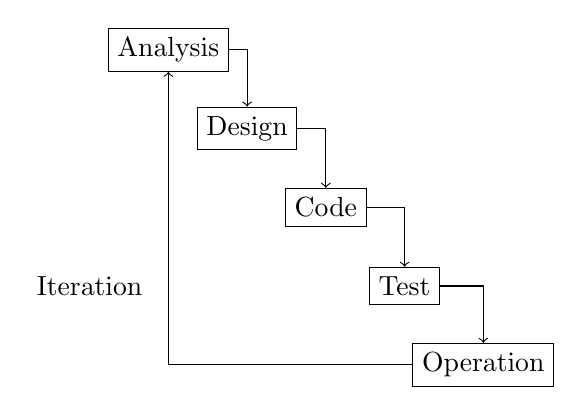
\begin{tikzpicture}
            % nodes
            \node (a1) [draw]  {Analysis};
            \node (d1) [draw, below of=a1, right of=a1] {Design};
            \node (c1) [draw, below of=d1, right of=d1] {Code};
            \node (t1) [draw, below of=c1, right of=c1] {Test};
            \node (o1) [draw, below of=t1, right of=t1] {Operation};
            \node at (-1,-3) {Iteration};
            % arrows
            \draw[->, to path={-| (\tikztotarget)}](a1) edge (d1) (d1) edge (c1) (c1) edge (t1) (t1) edge (o1) (o1) edge (a1);
        \end{tikzpicture}
        \caption{Incremental software development model life cycle}
        \label{fig:incremental-model}
    \end{figure}


\section{Version Control System}
When developing a software challenges can occur unexpectedly and a developer has to do whatever possible to ensure the their work is protected. For example, untraceable bug can be introduced in one of the iterations of the iterative development model (see section \ref{section:development-model}) that could lead to poor system performance. In order to prevent the (or at least dramatically lower)the occurrence these situations the use of \textit{"Version Control"} is encouraged.

There are many Version Control Systems (VCS) out there such as Mercurial, Fossil and Git. The main purpose of a \gls{vcs} is to keep track of the changes in a project. If a developer is satisfied with a specific change, they can perform a \textit{commit}. That action will merge the change to the codebase and the commit command will be added to the changelog (list of commits). If there is a problem that has been caused by a previous \textit{"bad"} commit, the developer can simply revert the whole project to a more stable state by restoring the codebase to a previous known \textit{"good"} commit.

For this project, Git has been chosen along with its web service GitHub\footnote{\url{https://github.com}} to serve as a \gls{vcs} due to the fact that it is easy to use and it is well-documented.

